\documentclass{article}
\usepackage{ctex}
\usepackage{geometry}
\geometry{top = 2cm, left = 1cm, right = 1cm, bottom = 2cm}
\usepackage{amsmath,amssymb,amsthm,amsfonts}
\usepackage{abstract}
\usepackage{siunitx}
\usepackage{graphicx}
\usepackage{booktabs}
\usepackage{appendix}
\usepackage{hyperref}
\usepackage{lscape}

\renewcommand{\appendixpagename}{附录}


\title{利用反符合法提高峰康比}
\author{钱思天 2001112187}
\begin{document}
    \maketitle
    \begin{abstract}
        本实验通过测量$N_c-t_d$曲线与效率曲线等,确定了实验中反符合的电子学参数。而后,通过分别测量是否存在反符合的$^{137}\text{Cs}$谱并进行峰康比计算,对反符合法对提升峰康比的效果进行了评估。
        \newline
        \newline
        {\emph{ 关键词:\ 反符合、$\gamma$射线谱、康普顿效应 }\rm}

    \end{abstract}

    \section{实验介绍}
    \subsection{实验原理}
    峰康比是表征$\gamma$射线谱仪性能的重要指标,其数值为全能峰峰道址计数与康普顿坪区平 均计数之比。它反应谱仪在存在高能强峰时分辨低能弱峰的能力,即当一个峰叠加在另一个 谱线的康普顿坪上时,该峰能否清晰地表现出来。峰康比越大,对复杂的$\gamma$谱越容易观察和 分析。

在闪烁体探测器中,闪烁晶体的大小是有限的,入射的$\gamma$光子在晶体中发生康普顿效应 时,有一部分康普顿散射光子可能会从晶体中逃逸出去。在这种情况下,探测器获得的能量 仅仅是康普顿反冲电子所获得的能量。由于反冲电子的能量随散射角大小而改变,其值为从 零到某一最大能量的连续分布,反映到能谱中,会形成一段比较平坦的连续谱,称为康普顿 坪。

康普顿坪的存在对多种能量$\gamma$射线的分辨和对$\gamma$射线强度的测量都是不利的因素。能量 较低的 $\gamma$ 射线的全能峰有可能被能量较高的 $\gamma$ 射线的康普顿坪淹没掉。故在复杂 $\gamma$ 能谱的测 量中,一定要设法提高峰康比,即尽可能提高全能峰计数,同时尽可能降低康普顿坪的计数。

将反符合屏蔽技术应用于 $\gamma$ 射线谱仪,是降低康普顿坪计数、提高峰康比、提高探测系 统性能的有效方法。它用反符合探测器探测那些逃逸出闪烁晶体的康普顿散射光子,跟主探 测器发生的康普顿效应事件进行反符合,可以剔除掉这些康普顿效应事件,达到降低康普顿 坪计数的目的。此外,在低水平 $\gamma$ 放射性测量装置中,为了降低本底计数,采用反符合法也 是一种有效措施。
    \subsubsection{$\gamma$射线的峰康比}
    在小体积晶体的单晶谱仪中,$\gamma$射线能量往往不能被全部吸收,大量康普顿散射光子会
逃逸出晶体,使康普顿坪区有较高的计数。当有多种能量的 $\gamma$ 射线入射时,低能 $\gamma$ 射线的全 能峰有可能被高能$\gamma$射线的康普顿坪所淹没,这对$\gamma$射线能量的分辨及他们相对强度的确定 都非常不利。

当 $\gamma$ 射线能量 $E_\gamma>2m_ec^2$ 时,除康普顿效应外,由电子对效应产生的单逃逸峰和双逃逸 峰,对多种能量 $\gamma$ 谱也将产生干扰。因此,在复杂 $\gamma$ 谱测量中要设法使全能峰尽量增高,而 使康普顿坪尽量降低,即提高 $\gamma$ 能谱的峰康比。

峰康比是 $\gamma$ 谱仪的重要性能指标之一,标志着谱仪分析复杂 $\gamma$ 谱的能力。一个带有反 符合屏蔽装置的全吸收谱仪是能够提高 $\gamma$ 能谱峰康比的。
\subsubsection{反符合法}
反符合法是用反符合电路来排除同时发生或有时间关联的事件。在反符合电路的两个输入信 号中,一个叫分析道,另一个叫反符合道,反符合道的脉冲作为消除符合事件的信号使用。

利用反符合屏蔽技术,将康普顿效应中反冲电子产生的脉冲作为分析道,将逃逸出
NaI(Tl)闪烁体并被反符合屏蔽探测器探测到的散射光子产生的脉冲作为反符合道,经过反 符合电路选择后就能把逸出光子事件消除掉。利用这种方法可以减少反冲电子产生的脉冲计 数,从而达到降低康普顿坪的目的。

\begin{figure}[htbp]
    \centering
    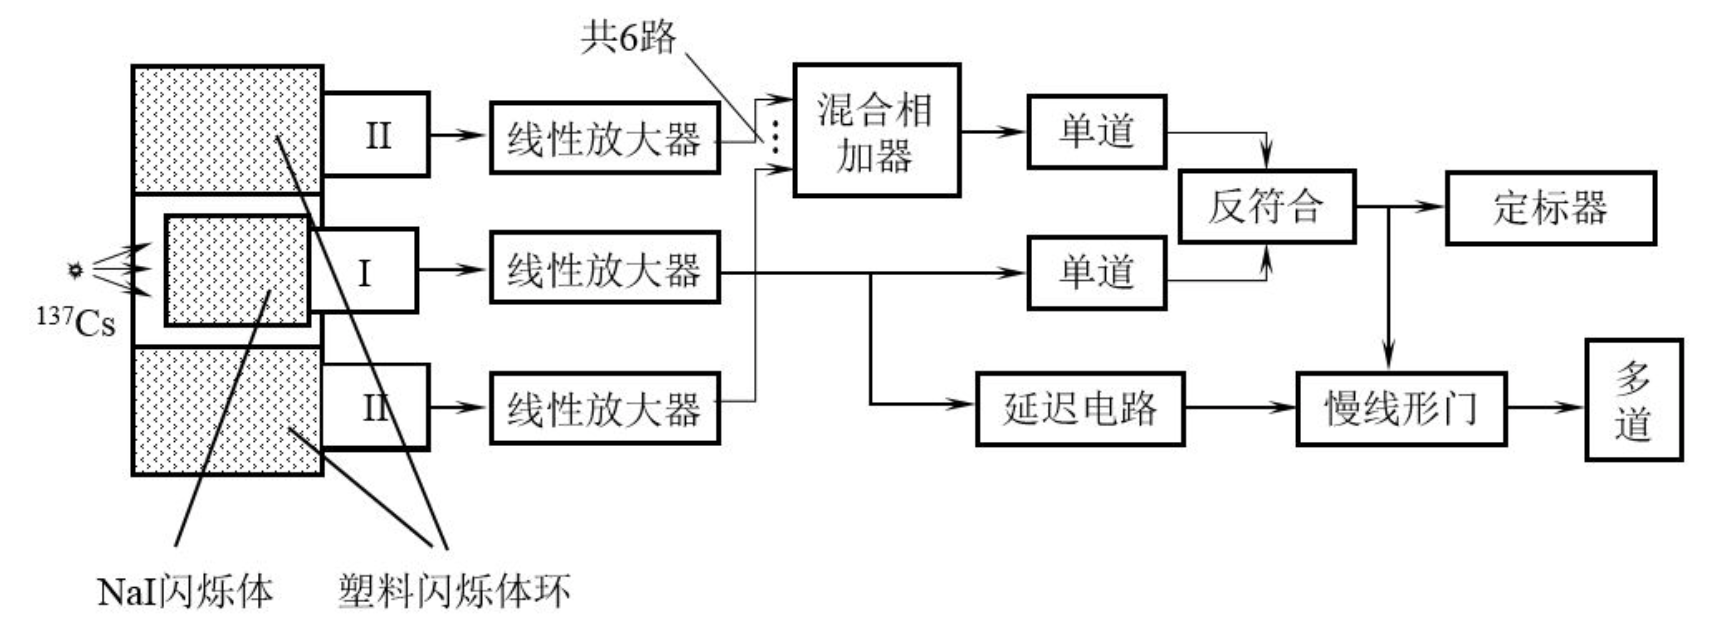
\includegraphics[width=\textwidth]{../plots/Anti_Co_Illus.png}
    \caption{反符合电路示意图\label{fig:Anti_Co_Illus}}
\end{figure}

反符合屏蔽全吸收谱仪的实验装置结构示意图如图\ref{fig:Anti_Co_Illus}所示。位于中间的探测器 I 为分析道探测器,称为主探测器,采用 NaI(Tl)闪烁体,用于探测 $\gamma$ 射线的能量。探测器 II 是 反符合屏蔽探测器,选用塑料闪烁体。塑料闪烁体为环状,包围在 NaI 晶体周围,沿塑料闪 烁晶体装置六个光电倍增管,构成探测器阵列,称为外围探测器。用于探测逃逸出 NaI 晶体 的散射光子,其输出信号经过放大、混合相加合并成一个信号,送入反符合道。

当 $\gamma$ 光子射入中央的主探测器时,若 $\gamma$ 光子的能量全部损耗在 NaI 晶体内,反符合道
没有信号而分析道有输入信号,反符合电路有信号输出。若 $\gamma$ 光子在主探测器内发生康普顿 效应,且康普顿散射光子从晶体中逸出后被外围探测器探测到,这时分析道和反符合道同时 有信号输入,反符合电路将没有信号输出。
将反符合输出脉冲输入慢线性门电路的门控输入端,作为开门信号,对来自主探测器 的分析脉冲进行选择,可以排除掉大部分逸出光子事件,从而降低了康普顿坪,提高了峰康 比。

\subsection{实验目的}
\begin{enumerate}
    \item 了解反符合方法的基本原理,及其在核物理实验中的应用。
    \item 用反符合屏蔽提高铯 137 伽马能谱的峰康比。
\end{enumerate}
\section{实验描述}
\subsection{实验装置}
实验装置较为复杂,其示意图基本如\ref{fig:Anti_Co_Illus}所示,除了我们实际上使用了5路外围放大器。实验装置列表如下:
\begin{enumerate}
    \item 主晶体-NaI(Tl)闪烁晶体,1 块; 
    \item 反符合晶体-环形塑料闪烁晶体,1 块; 
    \item 光电倍增管和前放,7 套。
    \item 高压电源,6 台; 
    \item 低压电源,2 台; 
    \item 线性放大器,5 台; 
    \item 定时单道分析器,2 台; 
    \item 反符合电路,1 台; 
    \item 慢线性门电路,1 台; 
    \item 延迟放大器,1 台; 
    \item 混合相加器,1 台;
    \item 定标器,1 台; 
    \item 多道脉冲分析器和打印机,1 套; 
    \item 示波器,1 台;
    \item 137Cs 放射源,1 个。
\end{enumerate}
\subsection{实验步骤}
\begin{enumerate}
    \item 调节主探测器的工作电压(${520\si{V}}$),并用示波器观察,使全能峰对应的脉冲信号
    幅度大约在$6\sim8\si{V}$。
    \item 调节各个反符合探头的高压,使定标器三秒计数为 25000 至 35000,
    要求高压不超过$1050\si{V}$(旋钮读数7.0) 。
    \item 调节反符合插件中主探测器信号和外围探测器信号的相对延迟时间,用定标器记录不同延迟时间下的反符合输出计数,测量$N_c-t_d$曲线,确定最佳的延迟时间。其中,将主信号的时间设置为$3.5\si{\micro s}$,而后调节外围放大器信号的延迟时间。
    \item 在 $0.1\si{V}$ 至 $0.5\si{V}$ 范围内改变单道阈值,根据反符合的效果,确定最佳的单道阈值。
    \item 把反符合输出信号作为慢线性门的“门输入”,经过延迟放大器的主探头信号作为慢
    线性门的“输入”。用双踪示波器观察,改变延迟放大器的延迟时间,把到达慢线性门的这 两路信号调成“同时”。
    \item 改变线性门宽度,观察信号有什么变化。选择适合的线性门宽度。
    \item 分别在有反符合和没有反符合的条件下测量$^{137}\text{Cs}$的$\gamma$能谱,每个测量 30 分钟。
\end{enumerate}
\section{实验数据}
\subsection{高压调节}
实验开始时,会调节各放大器的高压。在实际进行实验的时候,外围放大器的高压需要时不时进行调节\footnote{感谢赵捷老师的帮助},并且其计数也并不稳定。故在此并不记录各高压的数值。
\subsection{测量$N_c-t_d$曲线}
通过改变净延迟时间$t_d$,我们可以得到$30\si{s}$计数记录如表\ref{tab:Nc_td}和图\ref{fig:Nc_td}。
\begin{table}[htbp]
    \centering
    \caption{$30\si{s}$计数记录表\label{tab:Nc_td}}
    \begin{tabular}{rrrrrrrrrrr}
\toprule
Up    &       1.0 &       1.1 &       1.2 &       1.3 &       1.4 &       1.5 &       1.6 &       1.7 &       1.8 &       1.9 \\       
Down  &       3.5 &       3.5 &       3.5 &       3.5 &       3.5 &       3.5 &       3.5 &       3.5 &       3.5 &       3.5 \\
Net   &       2.5 &       2.4 &       2.3 &       2.2 &       2.1 &       2.0 &       1.9 &       1.8 &       1.7 &       1.6 \\
Count &  194917.0 &  193515.0 &  194904.0 &  194640.0 &  191838.0 &  188047.0 &  181640.0 &  180290.0 &  179303.0 &  180294.0 \\
\midrule
2.0 &       2.1 &       2.2 &       2.3 &       2.4 &       2.5 &       2.6 &       2.7 &       2.8 &       2.9 &       3.0 \\
3.5	&		3.5 &       3.5 &       3.5 &       3.5 &       3.5 &       3.5 &       3.5 &       3.5 &       3.5 &       3.5 \\
1.5 &       1.4 &       1.3 &       1.2 &       1.1 &       1.0 &       0.9 &       0.8 &       0.7 &       0.6 &       0.5 \\
179759.0 &  180200.0 &  180061.0 &  180739.0 &  180457.0 &  181749.0 &  184455.0 &  191342.0 &  194814.0 &  195463.0 &  195422.0 \\
\bottomrule
\end{tabular}

\end{table}
\begin{figure}[htbp]
    \centering
    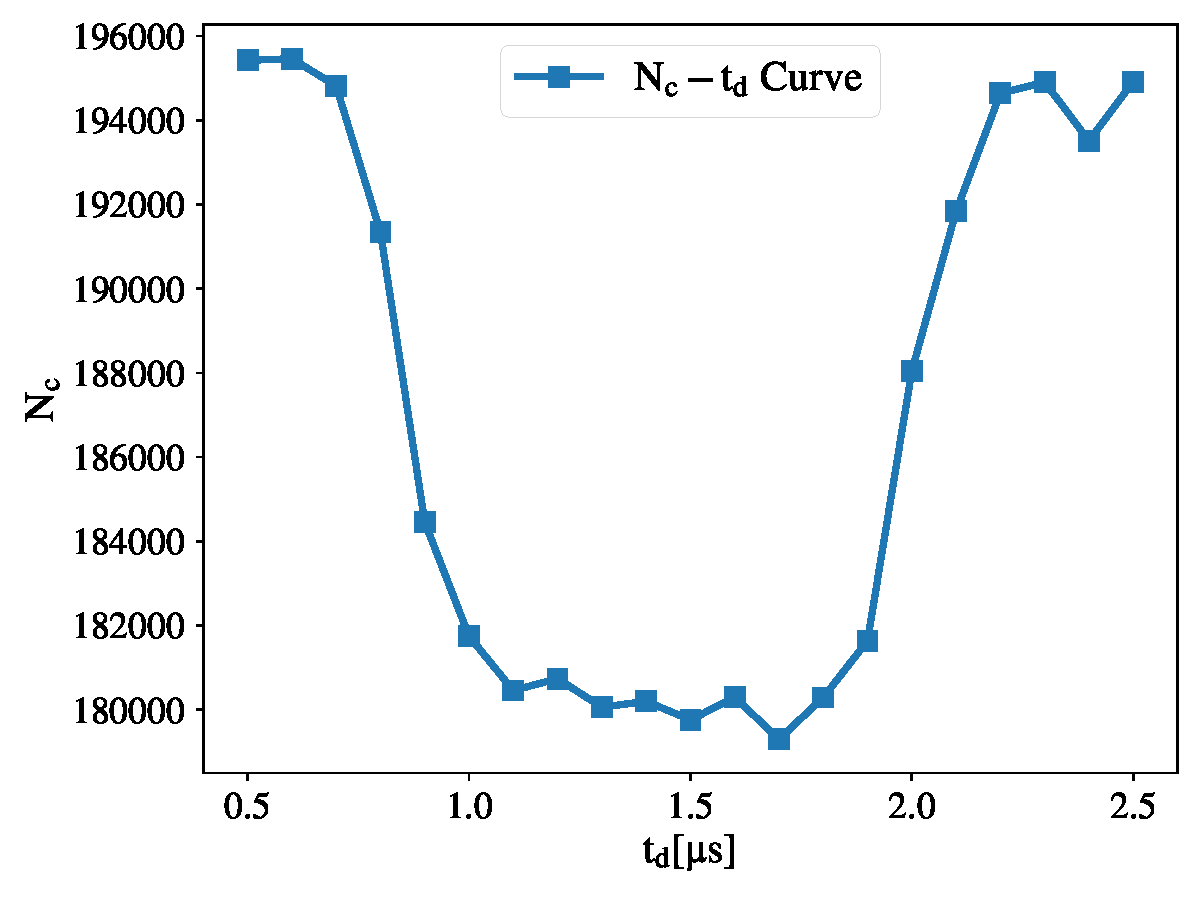
\includegraphics[width=0.7\textwidth]{../plots/Nc_td.pdf}
    \caption{$N_c-t_d$曲线\label{fig:Nc_td}}
\end{figure}
    
根据曲线\ref{fig:Nc_td},确定
\begin{equation}
    \begin{cases}
    t_{d1} = 0.85\si{\micro s}\\
    t_{d2}=2.0\si{\micro s}
    \end{cases}
\end{equation}得到\begin{equation}
    t_{d0} = 1.4\si{\micro s}
\end{equation}对应于上(外围放大器)延迟$2.1\si{\micro s}$,主放大器延迟$3.5\si{\micro s}$。
\subsection{确定单道阈值}
对于单道阈值的确定,采用的方案是测量延迟时间差为$1.4\si{\micro s}$和$2.5\si{\micro s}$下的计数$N_0,N_3$并计算效率。测量如表\ref{tab:Eff}
\begin{table}[htbp]
    \centering
    \caption{单道阈值测量确定\label{tab:Eff}}
    \begin{tabular}{lrrrrr}
\toprule
Threshold[V] &       0.1 &       0.2 &       0.3&       0.4 &       0.5\\
$N_0$           &  180200 &  179854 &  171788 &  167257 &  169594 \\
$N_3$           &  195422 &  194110 &  183756&  174642 &  171049 \\
$(N_3-N_0)/N_3$   &       0.077893 &       0.073443 &       0.06513 &       0.042287 &       0.008506 \\
\bottomrule
\end{tabular}

\end{table}
\begin{figure}[htbp]
    \centering
    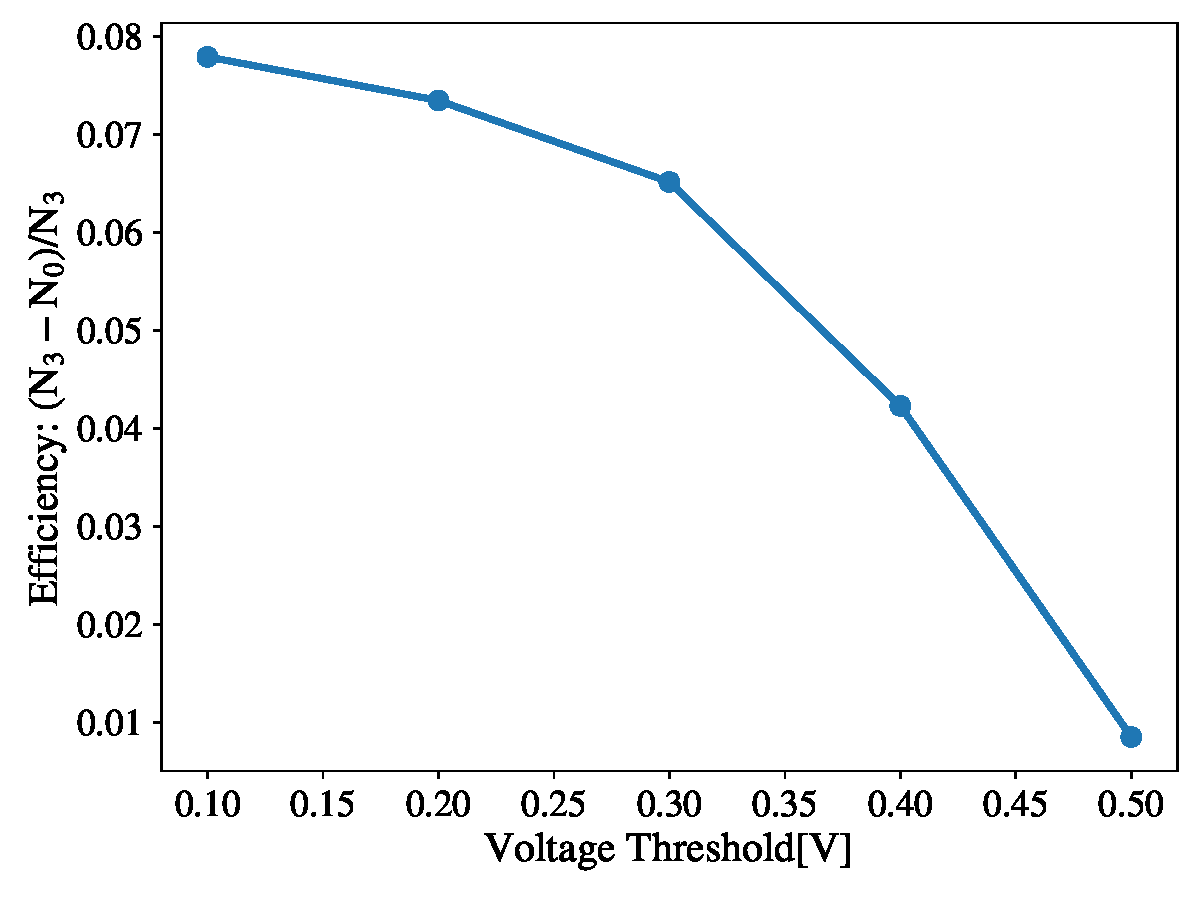
\includegraphics[width=0.7\textwidth]{../plots/Efficiency.pdf}
    \caption{单道阈值测量确定表\label{fig:Eff}}
\end{figure}

通过测量数据,确定阈值为$0.1\si{V}$。
\subsection{确定延迟放大器延迟时间和慢线性门门宽}
通过实验步骤中所叙述的方法,确定参数如下:
\begin{enumerate}
    \item 延迟放大器延迟时间:$1.2\si{\micro s}$;
    \item 慢线性门门宽:$5\si{\micro s}$。
\end{enumerate}
\subsection{$^{137}\text{Cs}$能谱测量}


\section{致谢}
    非常感谢赵捷老师的实验指导,也非常感谢和童星昱同学的讨论。
    \clearpage
    \appendix
    \appendixpage
    \section{思考题}
    \begin{enumerate}
        \item 提高伽马能谱的峰康比后,可以有效提高存在高能强峰时探测低能弱峰的能力。即如果低能弱峰落在高能强峰的康普顿坪上时,可以避免其被康普顿坪所
        淹没,使能谱更加干净。
        \item 通过设置阈值,卡掉全能峰。
        \item 偶然符合的计数率为
        \begin{equation}
            (N_1+N_2)-N_1N_2\tau
        \end{equation}
    \end{enumerate}
\end{document}